\documentclass[a4paper,12pt]{article}
\usepackage{graphicx}
\usepackage{titlesec}
\usepackage[utf8]{inputenc}
\usepackage{xcolor}
\usepackage{fancyhdr}
\usepackage{lipsum}
\usepackage{caption}

\renewcommand{\headrulewidth}{0pt}
\fancyhead[C]{}
\fancyhead[C]{
	
\includegraphics[width=4cm]{metu}
}
\pagestyle{plain}

%opening
\title{Middle East Technical University\\Department of Physics\\\textbf{PHYS307 Applied Modern Physics}}
\author{Oğuzhan ÖZCAN\\1852334}
\date{}
\clearpage
\thispagestyle{empty}
\providecommand{\groupmember}[1]{\textbf{Group Members:} }
\providecommand{\expdate}[1]{\textbf{Experiment Date:} }
\providecommand{\repdate}[1]{\textbf{Report Submit Date:} }
\providecommand{\expname}[1]{\textbf{Exp. MP-PE Photoelectric Effect} }


\usepackage[a4paper,%
left=0.5in,right=0.5in,top=0.5in,bottom=0.8in,%
footskip=.25in]{geometry}
%\topmargin -4.5cm
%\oddsidemargin 0.2cm
%\textwidth 16cm %
%\textheight 21cm%
%\footskip 1.0cm%




\begin{document}
\pagenumbering{gobble}
\maketitle

\thispagestyle{fancy}

%%%%%%%%%%%%%%%%%%%%%%%%%%%%%%%%%%%%%%%%%%%%%%%%%%%%%
\noindent\rule{18.4cm}{0.8pt}
\begin{center}
	\expname{arg1}{}
\end{center}
\groupmember{arg1}{Cem MADEN, İrem KÜL, Deniz AKYÜREK}\\
\expdate{November 6, 2015}{January 8, 2016}\\
\repdate{arg1}{January 15, 2016}\\
\noindent\rule{18.4cm}{0.8pt}\\\\
%%%%%%%%%%%%%%%%%%%%%%%%%%%%%%%%%%%%%%%%%%%%%%%%%%%%%
\begin{figure}[h!]
\centering
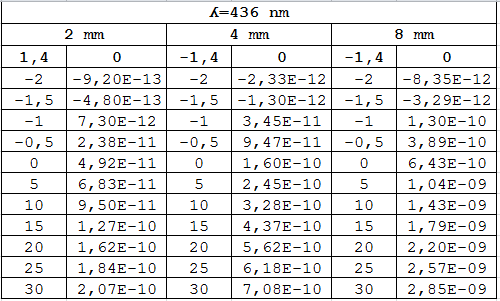
\includegraphics[scale = 0.7]{TABLE1}
\caption{Currents versus voltages for the light having constant wavelength at different intensities}
\label{fig:TABLE1}
\end{figure}
\begin{figure}[h!]
\centering
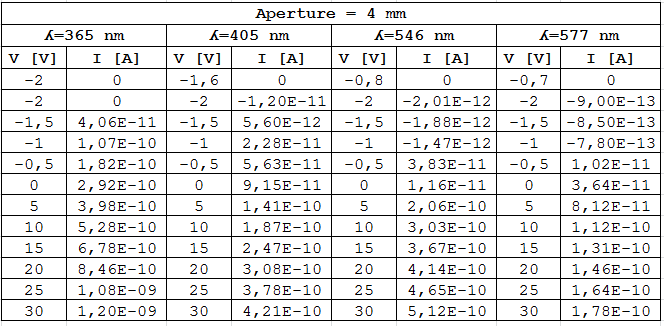
\includegraphics[scale = 0.7]{TABLE2}
\caption{Current versus voltages for the light having constant intensity at different wavelengths}
\label{fig:TABLE2}
\end{figure}
\newpage
\begin{table}[h!]

\begin{center}
	\begin{tabular}{|c|c|c|c|c|c|}
	\hline $\lambda$ [nm] & 365 & 405 & 436 & 546 & 577 \\ 
	\hline \textit{f} [$\times 10^{14}$ Hz] & 8.214 & 7.408 & 6.879 & 5.490 & 5.196 \\ 
	\hline $V_{0}$ [V] & -2.0 & -1.6 & -1.4 & -0.8 & -0.7 \\ 
	\hline 
\end{tabular} 
\end{center}
\caption{Stopping potentials versus different frequencies of light}
\end{table}

Apparent value of Planck Constant = 4.282$\times 10^{-15}$ eV$\cdot$s\\
Accepted value of Planck Constant = 4.135$\times 10^{-15}$ eV$\cdot$s\\
Work function = 1.5426\\
Percentage Error in Planck Constant =
\begin{equation}
P.E. = \frac{|4.135\times 10^{-15}-4.282\times 10^{-15}|}{4.135\times 10^{-15}}\times100=3.55\%
\end{equation}
\begin{figure}[h!]
\centering
\includegraphics[scale = 0.7]{"plot plancks constant"}
\caption{Plot of stopping potential versus frequency }
\label{fig:plotplancksconstant}
\end{figure}

\textbf{1. What is the most important general statement you can make from the results of your experiment?}\\\\
After this experiment, we state that light can behave as a particle. Besides, by using data that we took in experiment, we proved the Planck's Constant with an error lower than 5\%. Note that Plancks constant has two different values. In this experiment, we used in eV$\cdot$s unit.\\\\
\textbf{2. What are some advantages and disadvantages of the various yield characteristics (efficiencies) in Fig. PE.5.?}\\\\
In figure PE.5. there is three different phototubes. Since these phototubes have different properties, they have different curves. For instance, as stated in manual, S1 phototube is gas filled or S4 phototube is vacuum tube. By using different phototubes, we can observe different photoelectric efficiencies. Besides, modern phototubes are made with cesium antimonide surface.\\\\
\newpage
\textbf{3. Even if the bias voltage is zero, you can still measure a photocurrent. Explain why?}\\\\
Normally electrons collected in cathode. However, in this experiment, electrons are also collected in anode surface. That is why we measured some photocurrent when bias voltage is zero.\\\\
\textbf{4. When the anode is positive with respect to the cathode, why does not the current immediately rise to its saturation value? What happens to the electrons which do not reach anode?}\\\\
Stopping potential is the electrons whose do not reach to anode. When we applied negative potential to anode, then we have stopping potential. Current immediately rise to its saturation value if the voltage between the cathode and anode is greater than the stopping voltage, the photocurrent will increase quickly and eventually reach saturation.\\\\
\textbf{Discussion and Conclusion}\\\\
In this experiment we studied particle behaviour of light. We proved that light depends on energy and wavelength. In this experiment, we also stated the Planck's Constant with less than 5\% error. As we mentioned before, Planck's constant has different values for different units. Since we applied voltage and current, we found Planck's constant in eV$\cdot$s. 


















































































































































\end{document}
